\documentclass{hertieteaching}
\usepackage{pifont}
\usepackage{relsize}

\title{Content Analysis Dictionaries}

\begin{document}

\maketitle

% model structure choices
% preprocessing
% strategic considerations

\begin{frame}{Plan}
	

Dictionary based content analysis

The underlying measurement model

How to read a dictionary

Using the output

How to do it

How not to do it

Measurement error and its consequences
	
\end{frame}

\nocite{Monroe.etal2008,Robinson2016}

\begin{frame}{Classical dictionary content analysis}

\emph{Content} is, or is constructed from, \emph{categories} e.g.

\begin{itemize}
\item
  human rights, welfare state, national security
\end{itemize}

Substantively these often have \emph{valence}, e.g.

\begin{itemize}
\item
  pro-welfare state vs.~anti-welfare state, lots of CMP categories
\end{itemize}

But they are invariably treated as \emph{nominal level} variables

We are typically interested in them for

\begin{itemize}
\item
  simple descriptions, making comparisons, tracing temporal dynamics
\end{itemize}

\end{frame}

\begin{frame}{Talking like a newspaper}

{\centering 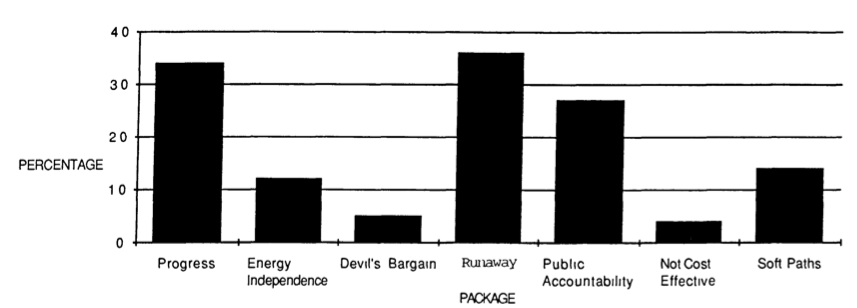
\includegraphics[width=0.9\linewidth]{pictures/gamson-modigliani-frames-opinion} 
}

\centerline{From \textcite{Gamson.Modigliani1989}}

\end{frame}

\begin{frame}{Talking like a presidential candidate}

\centerline{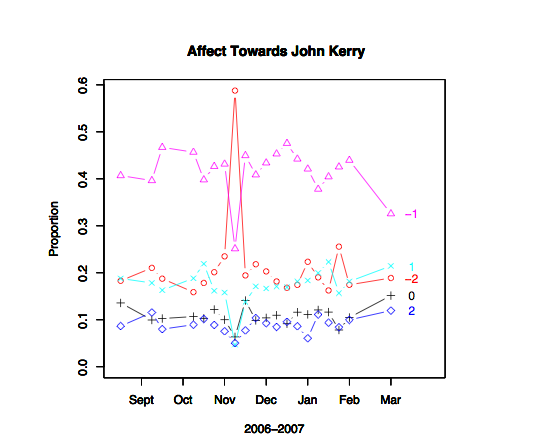
\includegraphics[width=0.55\linewidth]{pictures/kerry-blogs}} 

\centerline{From \textcite{Hopkins.King2010}}

\end{frame}

\begin{frame}{Talking like a terrorist}

\centerline{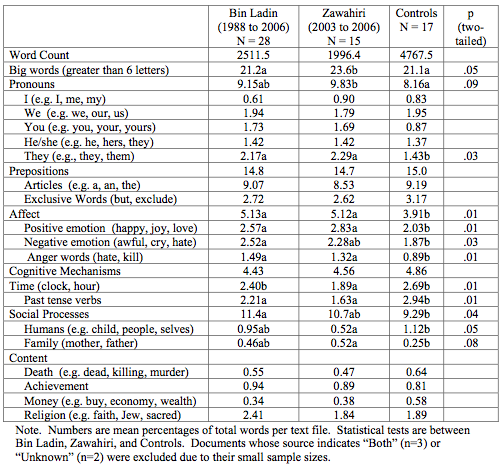
\includegraphics[width=0.6\linewidth]{pictures/binladen}} 

\centerline{From \textcite{Pennebaker.Chung2008}}

\end{frame}

\begin{frame}{Talking to police}


\centerline{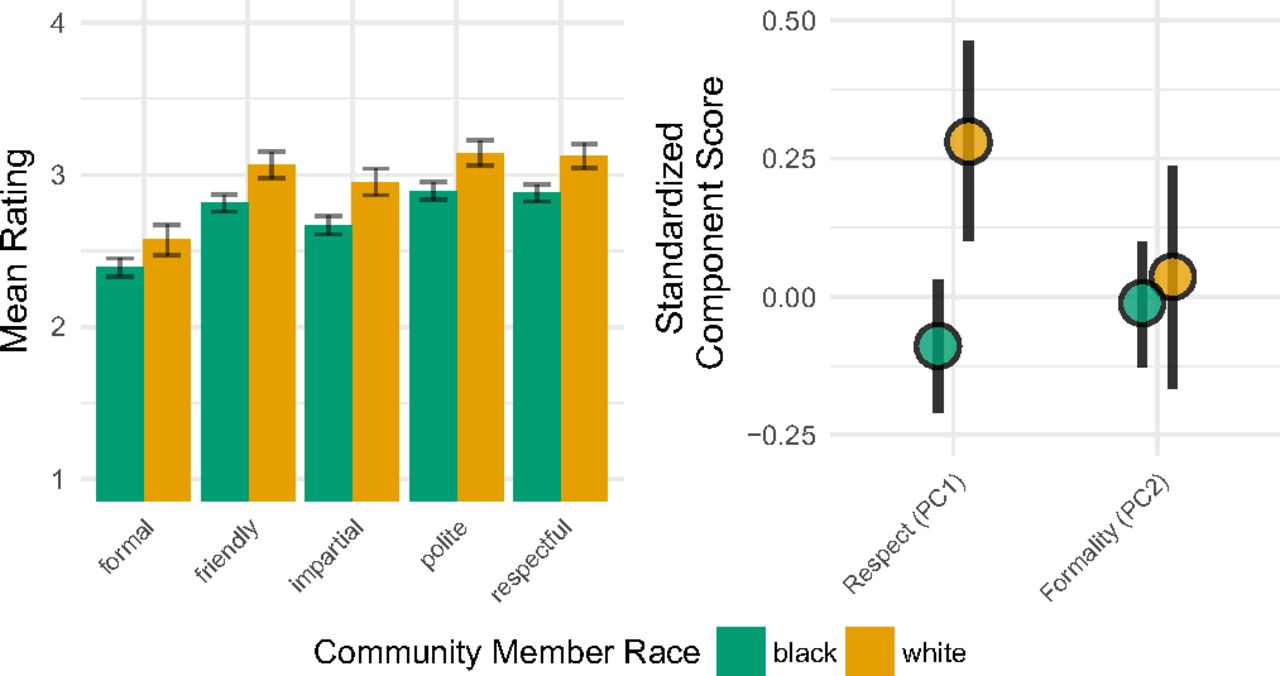
\includegraphics[width=0.7\linewidth]{pictures/respect.jpg}} 

\medskip
\centerline{From \textcite{Voigt.etal2017}}

\end{frame}

\begin{frame}{Classical content analysis}

Categories are
\begin{itemize}
\item
  equivalence classes over words\item
  representable as assignments of a K-valued category membership
  variable \(Z\) to each word
\end{itemize}

\begin{center}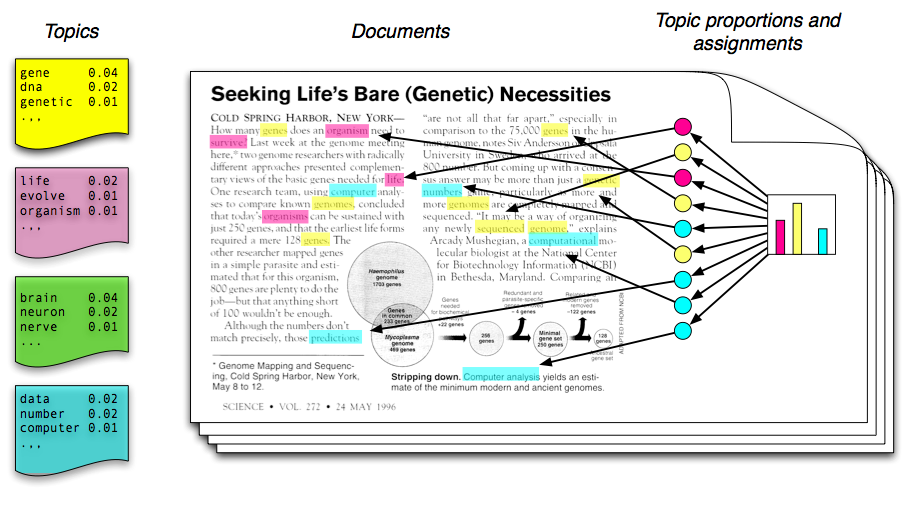
\includegraphics[width=0.6\linewidth]{pictures/topics2} \end{center}

\end{frame}

\begin{frame}{Topics}

\begin{columns}[T,onlytextwidth]
\column{0.5\textwidth}

\begin{center}
\begin{tikzpicture}
\node(W) at (1.5,0)  [var,label=below:$W$]{};
\pause
\node(Z) at (3,0)  [lat,label=below:$Z$]{};
\draw(Z) -- (W);
\pause
\draw[gray](1,-0.75) rectangle (3.75,0.5){};
\node[gray] at (4,-0.6){\small N};
\pause
\node(theta) at (4,1)  [lat,label=right:$\theta$]{};
\draw(theta) -- (Z);
\pause
\node(beta) at (-0.25, 0) [lat,label=below:$B$]{};
\draw(beta) -- (W);
\pause
\draw(-0.75,-0.75) rectangle (0.5,0.5)[gray];
\node(labk) at (-0.95,-0.6)  []{{\color{gray}\small K}};

\end{tikzpicture}
\end{center}

\column{0.05\textwidth}
\column{0.45\textwidth}

$W_i$ is the $i$-th word in the document
\medskip

$Z_i$ is true topic of $W_i$
\medskip

$\theta_k = P(Z = k)$ in this document
\medskip

$\beta_k$ in $B$ is the distribution $P(W \mid Z = k)$ 

\end{columns}

\end{frame}


\begin{frame}{Topics}

\begin{center}
\begin{tikzpicture}
\node(W) at (1.5,0)  [var,label=below:$W$]{};
\node(Z) at (3,0)  [lat,label=below:$Z$]{};
\draw(Z) -- (W);
\draw[gray](1,-0.75) rectangle (3.75,0.5){};
\node[gray] at (4,-0.6){\small N};
\node(theta) at (4,1)  [lat,label=right:$\theta$]{};
\draw(theta) -- (Z);
\node(beta) at (-0.25, 0) [var,label=below:$B$]{};
\draw(beta) -- (W);
\draw(-0.75,-0.75) rectangle (0.5,0.5)[gray];
\node(labk) at (-0.95,-0.6)  []{{\color{gray}\small K}};

\end{tikzpicture}
\end{center}


$B$ is a `dictionary' that explains how often each word should be generated in each of the $K$ topics
\begin{itemize}
  \item An entry in the dictionary $B$ is a vector of word generation probabilities $\beta_k$ 
\end{itemize}
This week we will assume we \textit{know} $B$

\pause
Strictly speaking we will assume that we know enough about its \textit{inverse} $W \longrightarrow Z$ to say
\begin{itemize}
  \item for each word $W$, what its $Z$ is.
\end{itemize}

\end{frame}

\begin{frame}{Dictionary B}

Here's a excerpt from the Economy section of the dictionary in \textcite{Laver.Garry2000}

\medskip
\begin{center}
\begin{tabular}{ll} \toprule
  \textbf{state reg}     & \textbf{market econ} \\ \midrule
          accommodation  & assets\\
          age            & bid\\
          ambulance      & choice*\\
          assist         & compet*\\
          benefit        & constrain*\\
          \ldots         & \ldots 
\end{tabular}
\end{center}

\end{frame}

\begin{frame}{How to read it}

Dictionary is an explicit and very \emph{certain} statement of
$P(Z \mid W)$

\begin{longtable}[]{@{}lll@{}}
\toprule
W & P(Z = `state reg' \textbar{} W) & P(Z = `market econ' \textbar{}
W)\tabularnewline
\midrule
\endhead
age & 1 & 0\tabularnewline
benefit & 1 & 0\tabularnewline
\ldots{} & \ldots{} & \ldots{}\tabularnewline
assets & 0 & 1\tabularnewline
bid & 0 & 1\tabularnewline
\ldots{} & \ldots{} & \ldots{}\tabularnewline
\bottomrule
\end{longtable}

\end{frame}

\begin{frame}{If we're so sure about $Z$\ldots}

Then estimating the proportion $Z=k$ in a document is easy.

First count up all the `hits', where $Z=k$
$$
Z_k ~=~ \sum^N_{i} P(Z = k \mid W_i)
$$
then divide by the sum
$$
\hat{\theta}_k ~=~ \frac{Z_k}{\sum^K_{j} Z_j}
$$
and that's our estimate of the document content
\end{frame}

\begin{frame}{Discrimination}

Stating $P(Z \mid W)$ is the \textit{discrimination} direction from last week
\begin{itemize}
  \item we didn't even learn it from data, we just asserted it!
\end{itemize}

So what must the generation process have looked like? 
\pause

The \emph{only} way this could be true is if the data had been generated
like

\begin{longtable}[]{@{}lll@{}}
\toprule
& state reg & market econ\tabularnewline
\midrule
\endhead
P(W = ``age'' \textbar{} Z) & a & \textbf{0}\tabularnewline
P(W = ``benefit'' \textbar{} Z) & b & \textbf{0}\tabularnewline
\ldots{} & \ldots{} & \ldots{}\tabularnewline
& &\tabularnewline
P(W = ``assets'' \textbar{} Z) & \textbf{0} & c\tabularnewline
P(W = ``bid'' \textbar{} Z) & \textbf{0} & d\tabularnewline
\ldots{} & \ldots{} & \ldots{}\tabularnewline
%\bottomrule
\end{longtable}

for arbitrary probabilities $a,b,c,d$. The real information in this dictionary is which words \textit{cannot} be generated by a topic

\end{frame}

\begin{frame}{Reconstruction}

Why do we seem to be going about this backwards?
\begin{itemize}
  \item Because we are reconstructing old practice as a measurement process
  \item which allows us to learn from data things we previously only asserted
  \item and understand exactly where and when things go wrong
\end{itemize}

But let's see how to work with the \textit{output} of the process before looking into its quirks

\end{frame}

\begin{frame}{Connecting content to politics}

We're usually interested in category proportions per unit (usually
document), e.g.

\begin{itemize}
\item
  \emph{How much} of this document is about national defense?\item
  What is the \emph{difference} of aggregated left and aggregated right
  categories (RILE)\item
  How does the \emph{balance} of human rights and national defense
  change over time?
\end{itemize}

\end{frame}

\begin{frame}{Inference about content}
\protect\hypertarget{inference-about-content}{}

Statistically speaking, we are just dealing with proportions of various
kinds

\begin{itemize}
\item
  a proportion\item
  a difference of proportions\item
  a ratio of proportions
\end{itemize}

Under certain sampling assumptions we can make inferences about a
population

\end{frame}

\begin{frame}{Simple inference about proportions}
\protect\hypertarget{simple-inference-about-proportions}{}

Example: in the 2001 Labour manifesto there are 872 matches to Laver and
Garry's \emph{state reg} category

\begin{itemize}
\item
  0.029 (nearly 3\%) of the document's words\item
  0.066 (about 6\%) of words that matched \emph{any} categories
\end{itemize}

The document has 30157 words, so the \emph{first} proportion is
estimated as

\[
\hat{\theta}_\text{\textsl{state reg}} ~=~ 0.029 ~~[0.027, 0.030]
\]

What does this mean?

\end{frame}

\begin{frame}{Inference about proportions}
\protect\hypertarget{inference-about-proportions}{}

Think of the party headquarters repeatedly \emph{drafting} this
manifesto

The true proportion -- the one suitable to the party's policies -- is
fixed but every draft is slightly different

The confidence interval reflects the fact that we expect long manifestos
to have more precise information about policy

\pause

This interval is computed as if

\begin{itemize}
\item
  every word was a new independent piece of information\item
  we're never wrong about word categories
\end{itemize}

\end{frame}

\begin{frame}{Ratios: How new was `New Labour'?}
\protect\hypertarget{ratios-how-new-was-new-labour}{}

Was the Conservative party in 1992 more or less for state intervention
than `New' Labour in 1997?

Compare instances of \emph{state reg} and \emph{market econ} in the
manifestos

\begin{longtable}[]{@{}lll@{}}
\toprule
party & \emph{state reg} & \emph{market econ}\tabularnewline
\midrule
\endhead
Conservative & 320 & 643\tabularnewline
Labour & 396 & 268\tabularnewline
\bottomrule
\end{longtable}

\end{frame}

\begin{frame}{Quantities of interest: Risk ratios}
\protect\hypertarget{quantities-of-interest-risk-ratios}{}

Compute two \emph{risk ratios}:

\[
\begin{aligned}
RR_{\text{\textsl{state reg}}} & ~=~ \frac{P(\text{\textsl{state reg}} \mid \text{cons})}
{P(\text{\textsl{state reg}} \mid \text{lab})}\\
RR_{\text{\textsl{market econ}}} & ~=~ \frac{P(\text{\textsl{market econ}} \mid \text{cons})}
{P(\text{\textsl{market econ}} \mid \text{lab})}
\end{aligned}
\]

and 95\% confidence intervals

\end{frame}

\begin{frame}{Interpreting risk ratios}
\protect\hypertarget{interpreting-risk-ratios}{}

If \(RR=1\) then the category occurs at the same rate in labour and
conservative manifestos

If \(RR=2\) then the conservative manifesto contains \emph{twice} as
much \emph{state reg} language as the labour manifesto

If \(RR=.5\) then the conservative manifesto contains \emph{half} as
much \emph{state reg} language as the labour manifesto

If the confidence interval for \(RR\) contains 1 then we \emph{no
evidence} that \emph{state reg} and \emph{market econ} occur at
different rates

\end{frame}

\begin{frame}{Risk ratios}
\protect\hypertarget{risk-ratios}{}

\begin{longtable}[]{@{}ll@{}}
\toprule
& Risk Ratio\tabularnewline
\midrule
\endhead
\emph{market econ} & 1.45 {[}1.26, 1.67{]}\tabularnewline
\emph{state reg} & 0.49 {[}0.42, 0.57{]}\tabularnewline
\bottomrule
\end{longtable}

Conservative manifesto generates \emph{market econ} words 45\% more
often

\begin{itemize}
\item
  45\% = 100(1.45 - 1)\%
\end{itemize}

Conservative manifesto only generates 49\% as many \emph{state reg}
words as Labour. Equivalently Labour generates them about \emph{twice}
as often

\end{frame}

\begin{frame}{Log ratios}
\protect\hypertarget{log-ratios}{}

It's often more useful to work with log ratios \[
\begin{aligned}
\text{log}(2)   & \approx 0.69\\
\text{log}(0.5) & \approx -0.69
\end{aligned}
\] which are

\begin{itemize}
\item
  symmetric, with an interpretable 0\item
  proportional (percentage increase/decreases)
\end{itemize}

\end{frame}

\begin{frame}{Log ratios as forensics (Robinson 2016)}
\protect\hypertarget{log-ratios-as-forensics}{}

\begin{figure}

{\centering 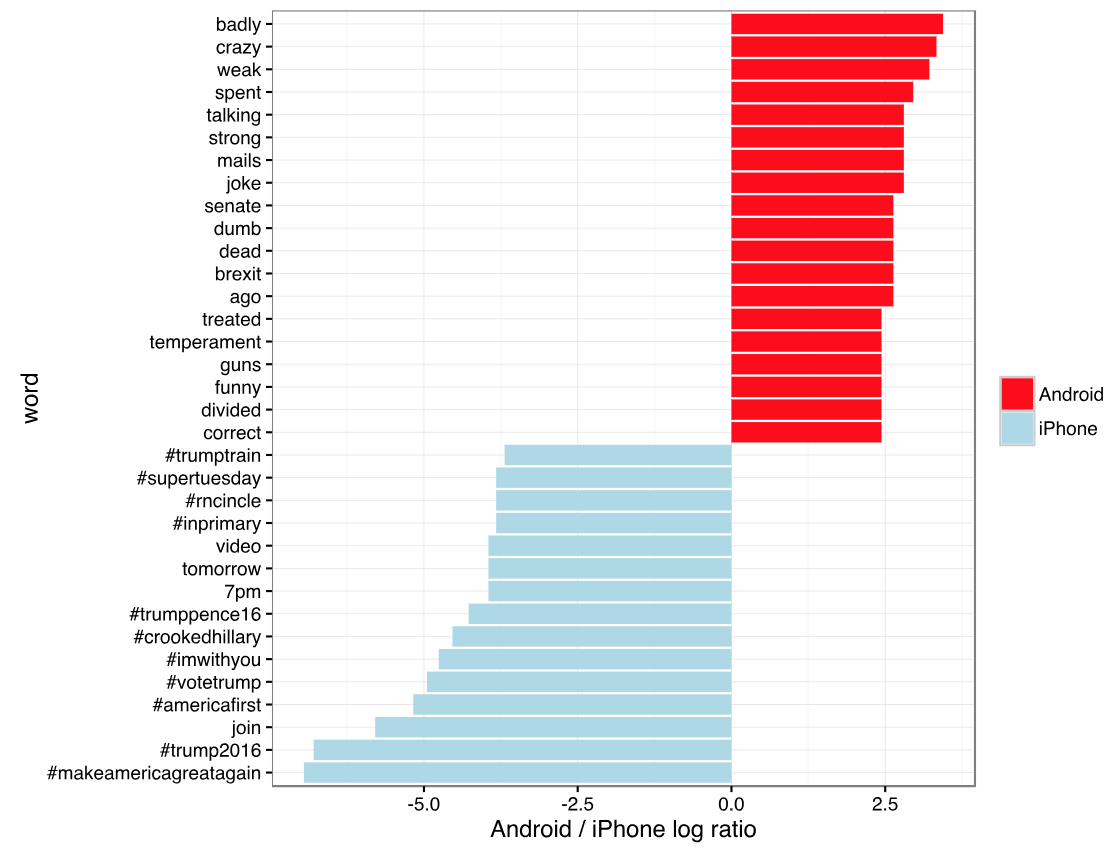
\includegraphics[width=0.6\linewidth]{pictures/trumptweets} 

}

\caption{David Robinson (2016)}\label{fig:unnamed-chunk-9}
\end{figure}

\end{frame}

\begin{frame}{Log ratios of words: (Monroe et al. 2008)}
\protect\hypertarget{log-ratios-of-words-keyness}{}

\begin{figure}

{\centering 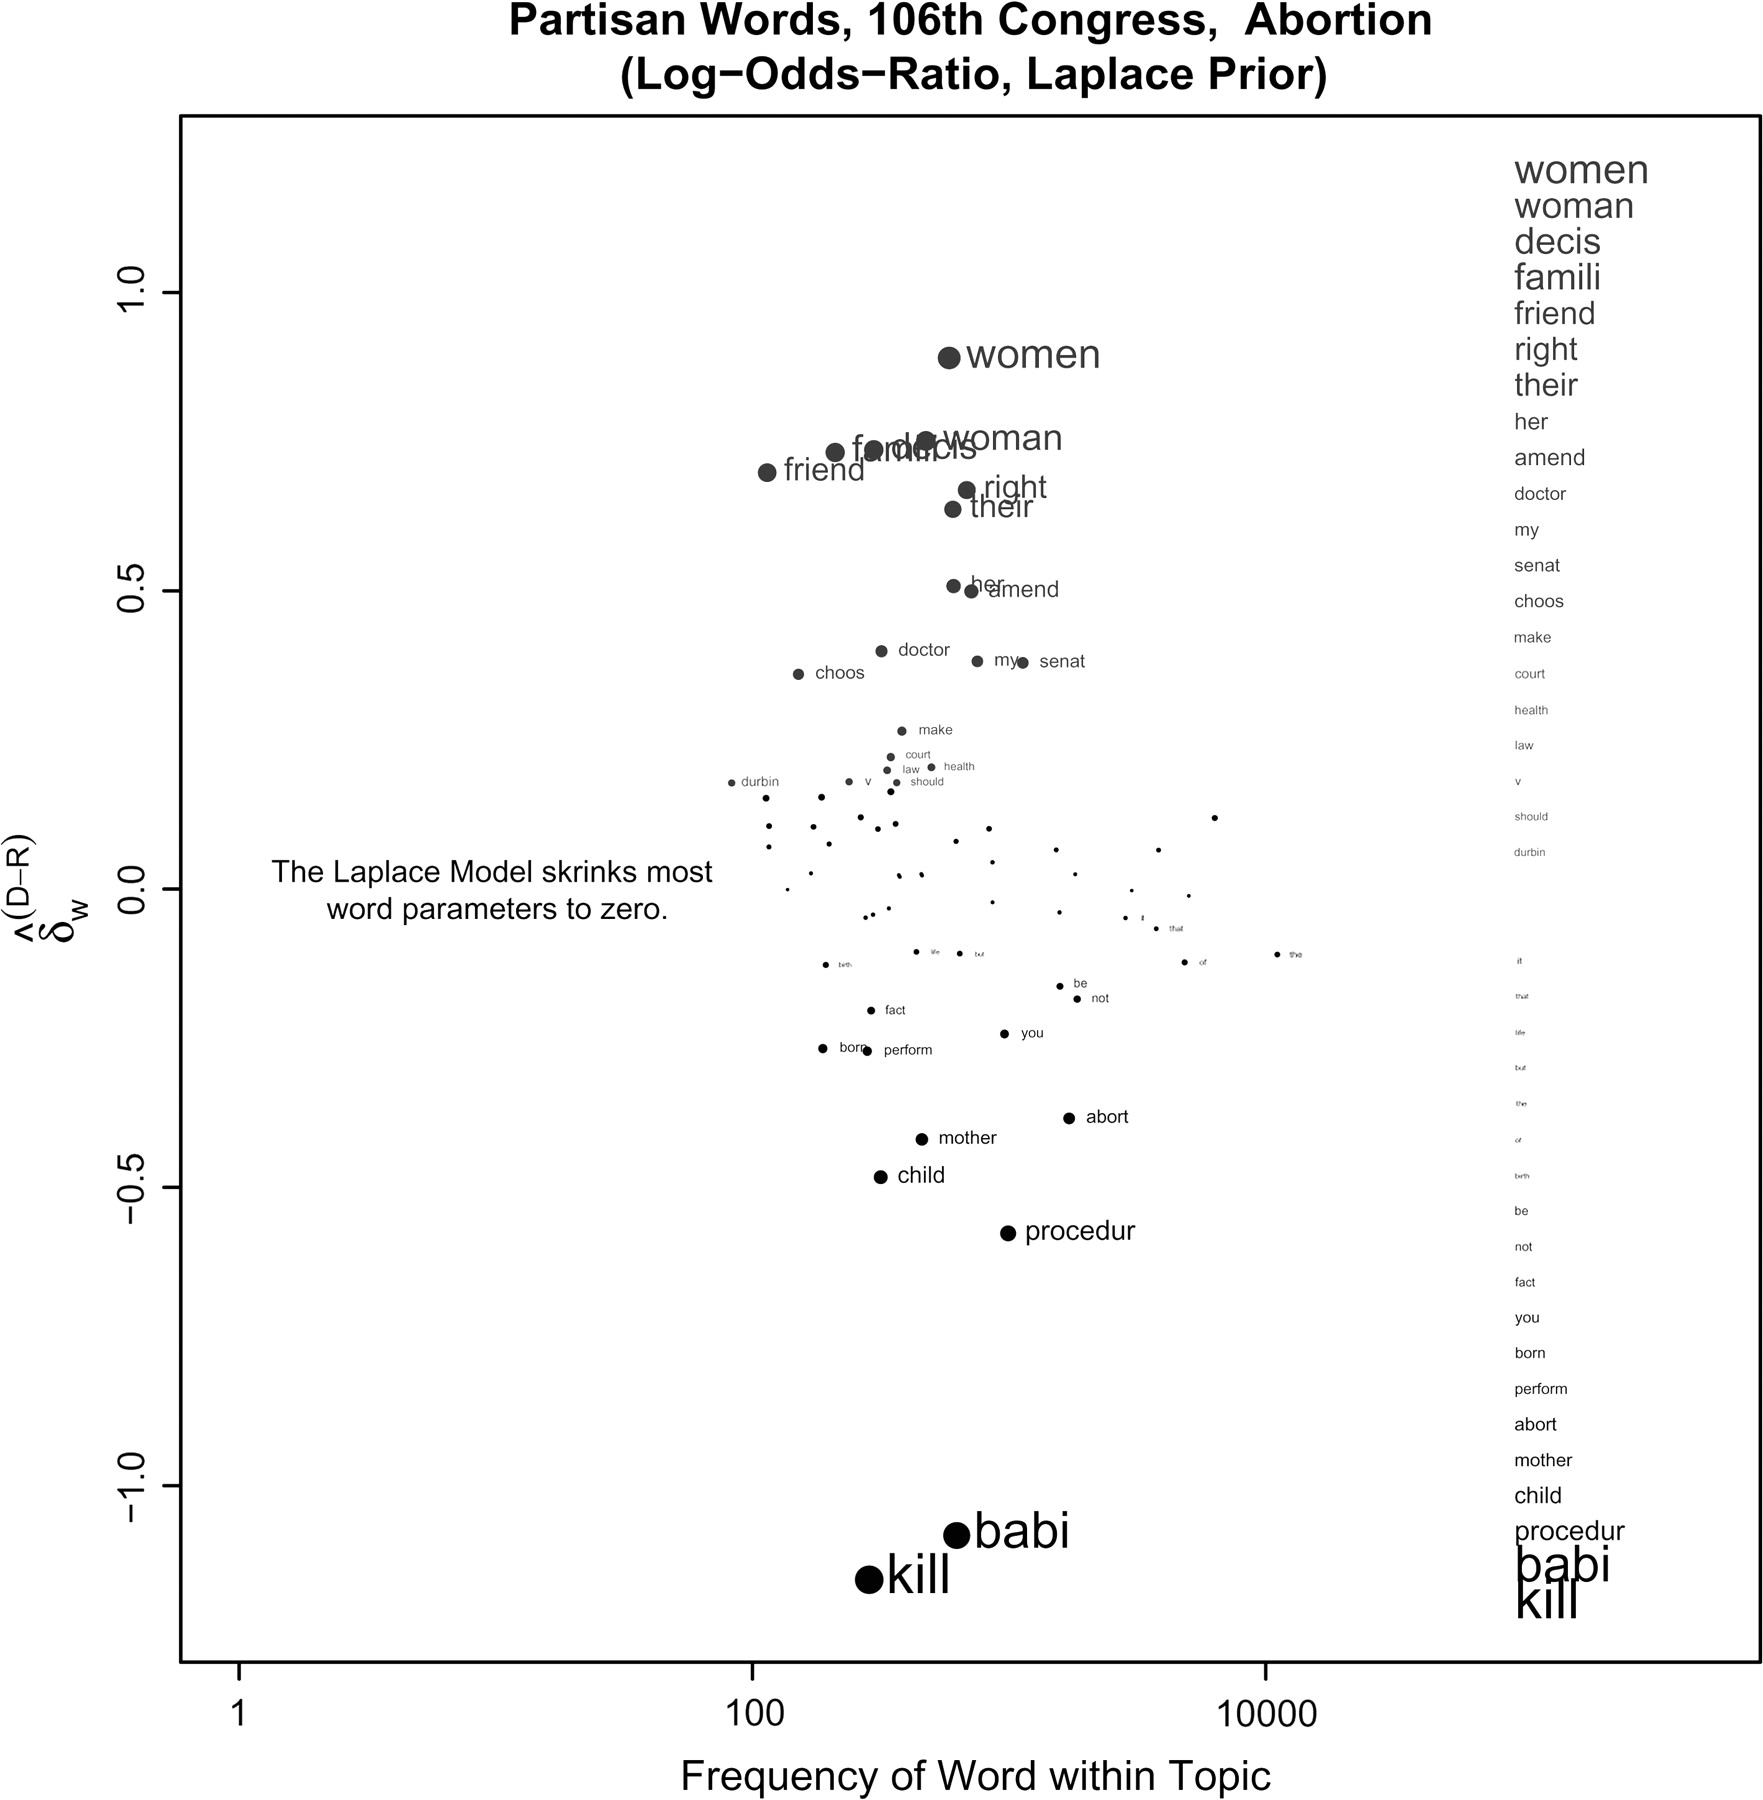
\includegraphics[width=0.6\linewidth]{pictures/fightin1} 

}

\caption{Monroe et al. (2008)}\label{fig:unnamed-chunk-10}
\end{figure}

\end{frame}

%\begin{frame}{Ratios, ratios everywhere}
%\protect\hypertarget{ratios-ratios-everywhere}{}
%
%\begin{longtable}[]{@{}lll@{}}
%\toprule
%party & \emph{state reg} & \emph{market econ}\tabularnewline
%\midrule
%\endhead
%Conservative & 320 & 643\tabularnewline
%Labour & 396 & 268\tabularnewline
%\bottomrule
%\end{longtable}
%
%Looking forward a little, there are two separate sorts of information in
%tables like these
%
%Marginal information:
%
%\begin{itemize}
%\item
%  e.g.~state regulation is mentioned 320+396=716 times, and market
%  economy 643+268=911 times.
%\end{itemize}
%
%\end{frame}

%\begin{frame}{Ratios, ratios everywhere}
%\protect\hypertarget{ratios-ratios-everywhere-1}{}
%
%\begin{longtable}[]{@{}lll@{}}
%\toprule
%party & \emph{state reg} & \emph{market econ}\tabularnewline
%\midrule
%\endhead
%Conservative & 320 & 643\tabularnewline
%Labour & 396 & 268\tabularnewline
%\bottomrule
%\end{longtable}
%
%Association information:
%
%\begin{itemize}
%\item
%  conservatives mention state regulation 320/643 = about 50\% as much as
%  market economy\item
%  labour mentions it 396/268 = about 50\% more than market economy.
%\end{itemize}
%
%So the odds ratio (0.5 / 1.5) = about 0.33.
%
%This, plus the marginal information, \emph{completely characterizes}
%this table.
%
%\end{frame}
%
%\begin{frame}{A psychological aside}
%\protect\hypertarget{a-psychological-aside}{}
%
%Are people \emph{really} sensitive to these sorts of associational
%statistics?
%
%\pause
%
%It seems they are:
%
%\begin{itemize}
%\item
%  Even infants track conditional probabilities ({\textbf{???}})\item
%  Purely statistical textual measures recover Implicit Association Test
%  biases ({\textbf{???}})
%\end{itemize}
%
%\end{frame}
%
%\begin{frame}{Word embeddings}
%\protect\hypertarget{word-embeddings}{}
%
%Contextual similarity tracks real relations (as it must!)
%
%\begin{center}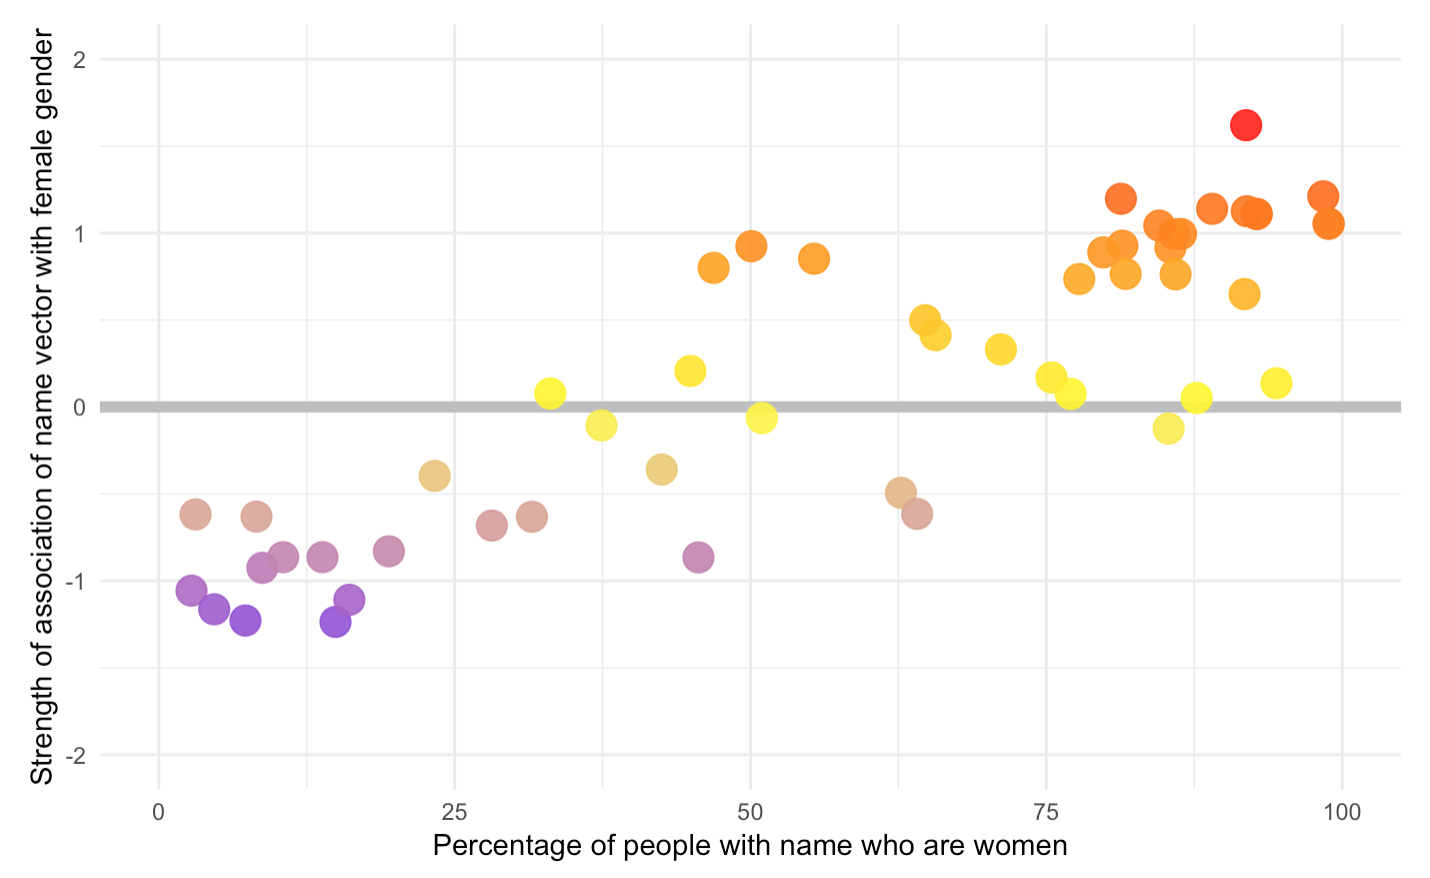
\includegraphics[width=0.9\linewidth]{pictures/cbn-jobs} \end{center}
%
%\end{frame}

\begin{frame}{Category count as a dependent variable}
\protect\hypertarget{category-count-as-a-dependent-variable}{}

\centerline{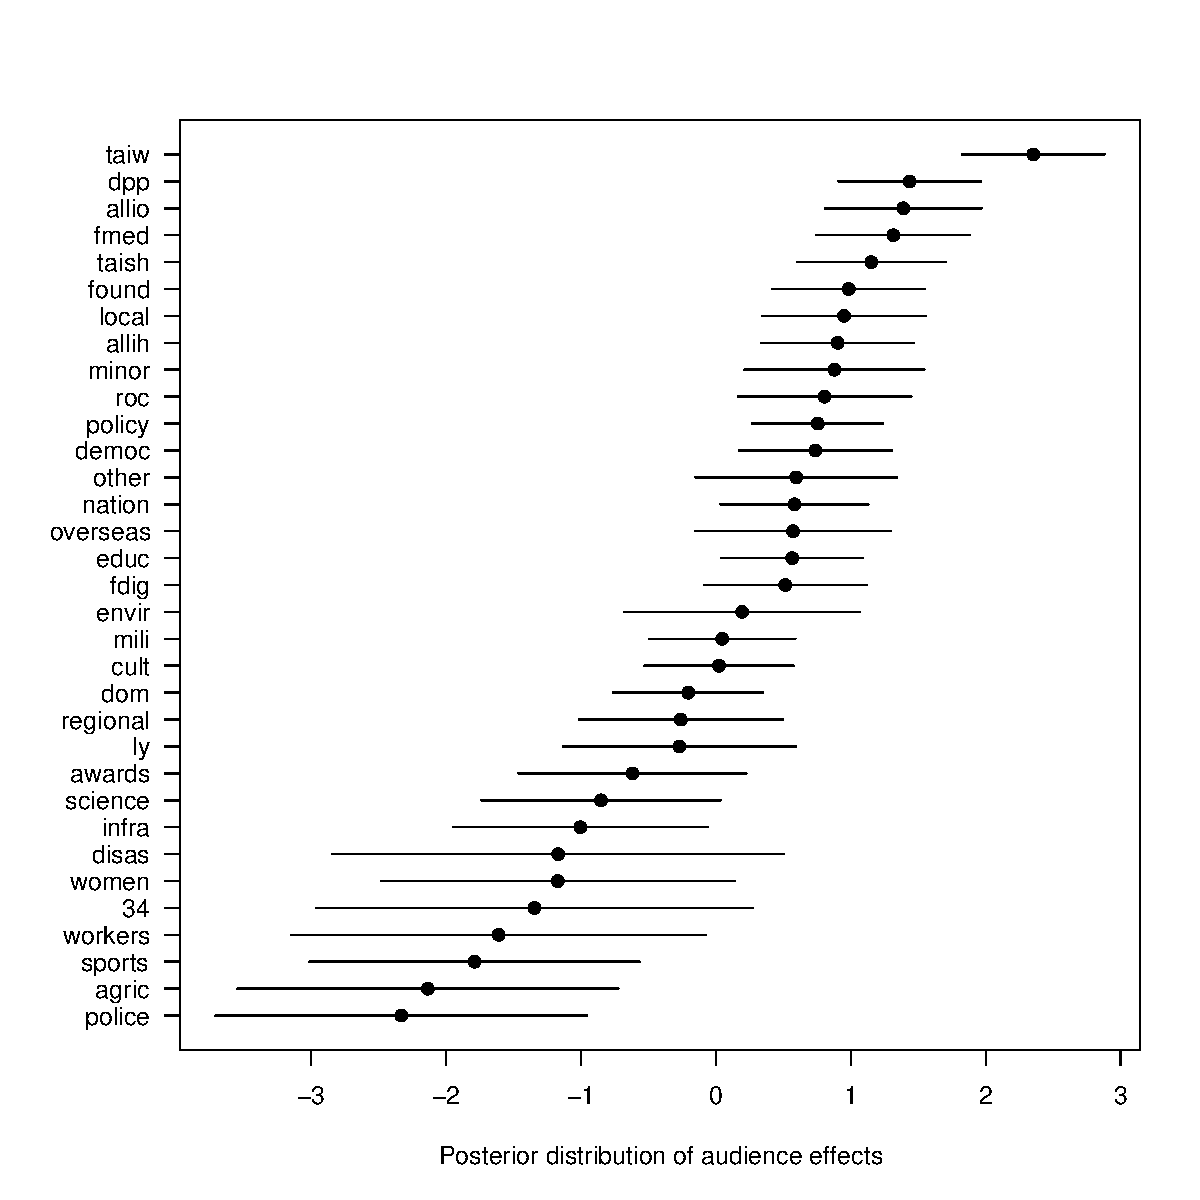
\includegraphics[width=0.5\linewidth]{pictures/indep-ref} }

From \textcite{Sullivan.Lowe2010}


\end{frame}

\begin{frame}{Category counts as a dependent variable}

District vs party focus in speeches

{\centering 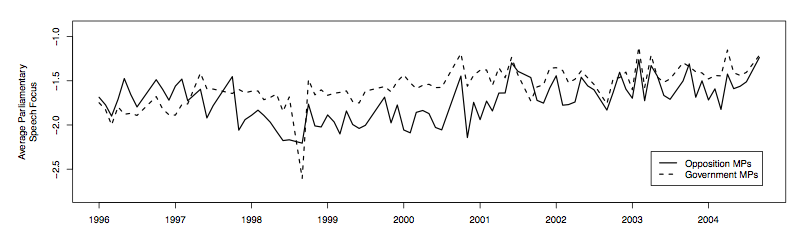
\includegraphics[width=0.9\linewidth]{pictures/district-party-focus} 

}
From Kellerman and Proksch, MS

%Data: {[}district words, party words{]}

\end{frame}

%\begin{frame}{Category counts as a dependent variable}
%\protect\hypertarget{category-counts-as-a-dependent-variable-1}{}
%
%Logit reminder:
%
%\begin{itemize}
%\item
%  when you are modeling two category counts as a function of covariates
%  the linear predictor is a smoothed version of their log ratio
%\end{itemize}
%
%\[
%\begin{aligned}
%\text{[dist, party]} & \sim \text{Binomial}(\pi^\text{dist}_, N_i)\\ 
%\text{log}\frac{\pi^\text{dist}_i}{(1 - \pi^\text{dist}_i)} & = \text{log}\frac{\pi^\text{dist}_i}{\pi^\text{party}_i} ~=~ \ldots 
%\end{aligned}
%\]
%
%\end{frame}

\begin{frame}{OK, how do I make such a dictionary?}

Find a suitable tool
\begin{itemize}
  \item \href{http://provalisresearch.com/products/content-analysis-software/}{Wordstat}
  \item \href{http://liwc.wpengine.com/}{LIWC} (maybe don't)
  \item \href{http://apb.newmdsx.com/hamlet2.html}{Hamlet}
  \item \href{http://atlasti.com/}{Atlas-ti} (?)
  \item \href{https://github.com/conjugateprior/yoshikoder/releases/tag/v0.6.5}{Yoshikoder}
\end{itemize}

\pause

Then assign words to
\begin{itemize}
\item
  maximise measurement validity
  \item
  minimise \emph{measurement error}
\end{itemize}

\pause

(Sell high, buy low)

\end{frame}

\begin{frame}{The source of measurement error}
\protect\hypertarget{the-source-of-measurement-error}{}

Measurement error in classical content analysis is primarily failure of
\emph{this} assumption:

\begin{longtable}[]{@{}lll@{}}
\toprule
W & P(Z = state reg \textbar{} W) & P(Z = market econ \textbar{}
W)\tabularnewline
\midrule
\endhead
age & 1 & 0\tabularnewline
benefit & 1 & 0\tabularnewline
\ldots{} & \ldots{} & \ldots{}\tabularnewline
assets & 0 & 1\tabularnewline
bid & 0 & 1\tabularnewline
\ldots{} & \ldots{} & \ldots{}\tabularnewline
\bottomrule
\end{longtable}

\end{frame}

\begin{frame}{Consequences of measurement error}
\protect\hypertarget{consequences-of-measurement-error}{}

What are the effects of measurement error in category counts?

Being directly wrong, e.g.

\begin{itemize}
\item
  Estimated rates are too \emph{low} (bias)\item
  Some of estimates are more biased than others
\end{itemize}

Being \emph{indirectly} wrong, e.g.

\begin{itemize}
\item
  Subtractive or ratio left-right measures are too \emph{centrist}
\end{itemize}

\end{frame}

\begin{frame}{Measurement error: example}
\protect\hypertarget{measurement-error-example}{}

Assume

\begin{itemize}
\item
  a vocabulary of only two words `benefit' and `assets'\item
  a \emph{subtractive} measure of position (Laver and Garry): \[
  \frac{Z_\text{market econ} - Z_\text{state reg}}
       {Z_\text{market econ} + Z_\text{state reg}}
  \]
\end{itemize}

Then we hope that the posterior over categories is:

\begin{longtable}[]{@{}llll@{}}
\toprule
& \emph{state reg} & \emph{market econ} &\tabularnewline
\midrule
\endhead
``benefit'' & 1 & 0 & 1\tabularnewline
``assets'' & 0 & 1 & 1\tabularnewline
\bottomrule
\end{longtable}

\end{frame}

\begin{frame}{Measurement error: example}
\protect\hypertarget{measurement-error-example-1}{}

but if word generation happened like this\ldots{}

\begin{longtable}[]{@{}lll@{}}
\toprule
& \emph{state reg} & \emph{market econ}\tabularnewline
\midrule
\endhead
``benefit'' & 0.7 & 0.2\tabularnewline
``assets'' & 0.3 & 0.8\tabularnewline
& &\tabularnewline
total & 1 & 1\tabularnewline
\bottomrule
\end{longtable}

then \[
P(W=\text{"asset"} |\mid Z=\text{state reg}) > 0
\]
so, e.g.
\[
P(Z=\text{state reg} \mid W=\text{"asset"}) < 1
\]

\end{frame}

\begin{frame}{Measurement error: example}
\protect\hypertarget{measurement-error-example-2}{}

Assume

\begin{itemize}
\item
  \(Z_{\text{\textsl{market econ}}} = 10\)\item
  \(Z_{\text{\textsl{state reg}}}=20\)
\end{itemize}

Then the \emph{true} difference is \[\frac{(10-20)}{(10+20)} = -0.33\]

Under perfect measurement we would expect

\begin{itemize}
\item
  20 'benefit's\item
  10 'assets's
\end{itemize}

\end{frame}

\begin{frame}{Measurement error: example}
\protect\hypertarget{measurement-error-example-3}{}

Under \emph{imperfect} measurement we expect

\begin{itemize}
\item
  16 `benefit' (14 from \emph{state reg} but 2 from \emph{market econ})\item
  14 `assets' (8 from \emph{market econ} but 6 from \emph{state reg})
\end{itemize}

The proportional difference measure is now \[
\frac{(14-16)}{(14+16)} = -0.07
\]

Apparently much closer to the centre, but only because of measurement
error

\pause

\emph{All} relative measures will have this problem (and all kinds of
text analyzers)

\end{frame}

\begin{frame}{In action (Laver and Garry 2000)}
\protect\hypertarget{in-action-laver-and-garry-2000}{}

{\centering 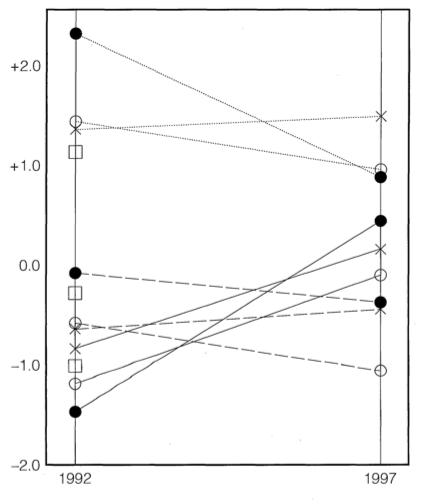
\includegraphics[width=0.4\linewidth]{pictures/lg-shrinkage} 

}

\end{frame}

\begin{frame}{In action with people, not dictionaries}

\begin{center}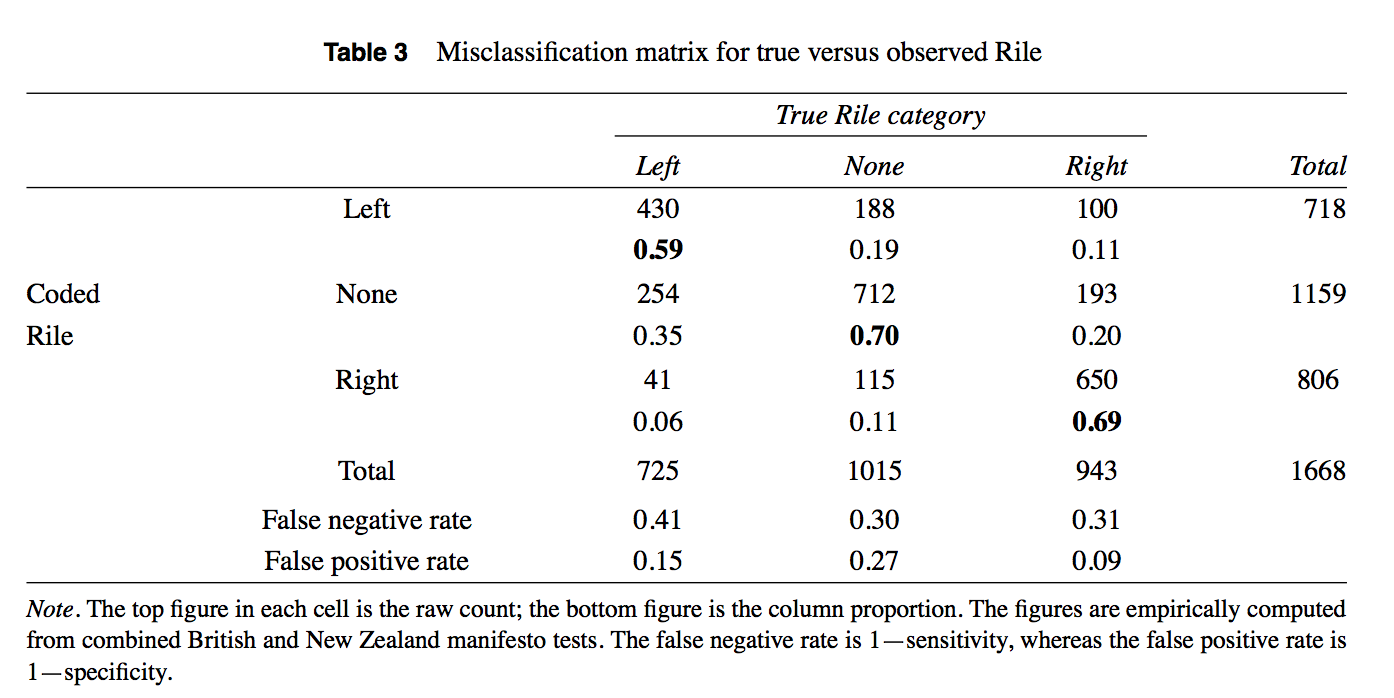
\includegraphics[width=0.8\linewidth]{pictures/slava-rile3} \end{center}

From \textcite{Mikhaylov.etal2011}

\end{frame}

\begin{frame}{So what to do now?}

That's for next week\ldots


\end{frame}
%\protect\hypertarget{solutions-some-theological-approaches}{}
%
%\pause
%
%\begin{figure}
%
%{\centering 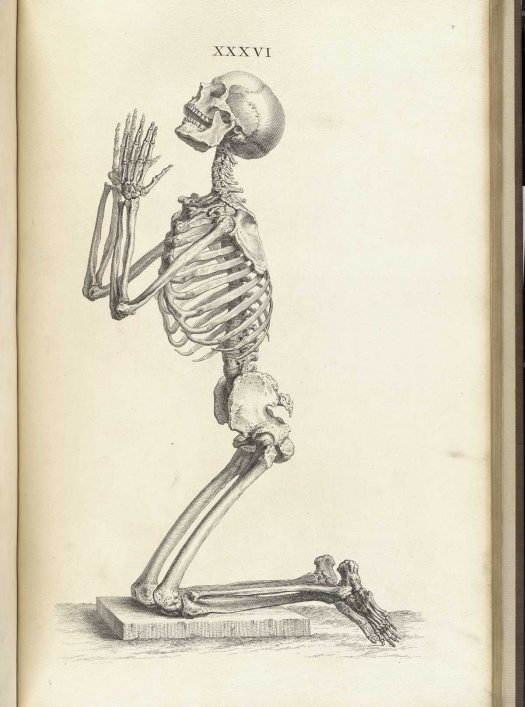
\includegraphics[width=7.29in,height=0.8\textheight]{pictures/praying-skeleton} 
%
%}
%
%\caption{Thoughts and Prayers}\label{fig:unnamed-chunk-18}
%\end{figure}
%
%\end{frame}
%
%\begin{frame}{Solutions: Do not sin in the first place}
%\protect\hypertarget{solutions-do-not-sin-in-the-first-place}{}
%
%``Beatings will continue until morale improves''
%
%\pause
%
%An often non-obvious fact about content dictionaries:
%
%\begin{itemize}
%\item
%  \emph{precision}: proportion of words used the way your dictionary
%  assumes\item
%  \emph{recall}: proportion of words used that way that are in your
%  dictionary
%\end{itemize}
%
%\emph{always} trade-off\ldots{}
%
%\end{frame}
%
%\begin{frame}{Sins of ommission vs sins of commission}
%\protect\hypertarget{sins-of-ommission-vs-sins-of-commission}{}
%
%Every field reinvents this distinction:
%
%\begin{itemize}
%\item
%  precision and recall\item
%  specificity and sensitivity\item
%  users and producer's accuracy\item
%  type 1 and type 2 error
%\end{itemize}
%
%\end{frame}
%
%\begin{frame}{Humility and self-examination}
%\protect\hypertarget{humility-and-self-examination}{}
%
%Keyword in context analyses (KWIC) allow you to scan all contexts of a
%word
%
%\begin{itemize}
%\item
%  How many of them are the sense or usage you want?
%\end{itemize}
%
%\end{frame}
%
%\begin{frame}{KWIC: \texttt{benefit*}}
%\protect\hypertarget{kwic-benefit}{}
%
%\tiny
%\begin{table}[ht]
%\centering
%\begin{tabular}{rlll}
%  \hline
% & pre & keyword & post \\ 
%  \hline
%1 & also keep all the other & benefits & that pensioners currently receive , \\ 
%  2 & regulation will have to have & benefits & exceeding costs , and regulations \\ 
%  3 & and Controlled Immigration Britain has & benefited & from immigration . We all \\ 
%  4 & positive contribution But if those & benefits & are to continue to flow \\ 
%  5 & Nor ther n Ireland brings & benefits & to all parts of our \\ 
%  6 & their home , will also & benefit & first-time buyers . Empowering individuals \\ 
%  7 & you help yourself ; you & benefit & and the country benefits . \\ 
%  8 & you benefit and the country & benefits & . So now , I \\ 
%  9 & result of our tax and & benefit & measures compared to 1997 . \\ 
%  10 & result of personal tax and & benefit & measures introduced since 1997 , \\ 
%  11 & , the savings on unemployment & benefits & will go towards investing more \\ 
%  12 & trebled the number on incapacity & benefits & . We will help 17 \\ 
%  13 & Work programme and reform Incapacity & Benefit & , with the main elements \\ 
%  14 & main elements of the new & benefit & regime in place from 2008 \\ 
%  15 & stronger penalties . To the & benefit & of business and household consumers \\ 
%  16 & effective directive to provide real & benefits & to consumers and new opportunities \\ 
%  17 & better.We are examining the potential & benefits & of a parallel Expressway on \\ 
%  18 & ways to lock in the & benefit & of new capacity . We \\ 
%  19 & are determined to spread the & benefits & of enterprise to every community \\ 
%  20 & to get ahead , to & benefit & from improving public services , \\ 
%  21 & of the school workforce is & benefiting & staff and helping to tailor \\ 
%  22 & teachers and pupils get the & benefit & of the range of support \\ 
%   \hline
%\end{tabular}
%\end{table}
%\normalsize
%
%\end{frame}
%
%
%
%\begin{frame}{Last week}
%\end{frame}

\begin{frame}[allowframebreaks]
\frametitle{References}
\printbibliography	
\end{frame}


\end{document}
